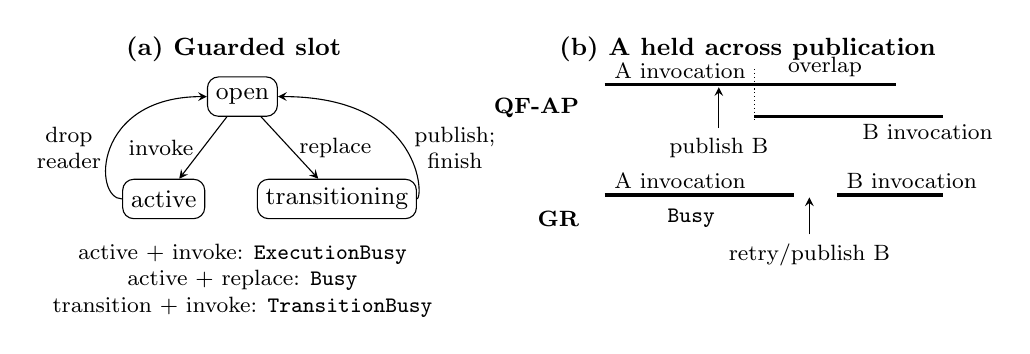
\begin{tikzpicture}[>=stealth, font=\small, state/.style={draw,rounded corners,minimum height=5mm,inner sep=3pt}]
\node[anchor=west,font=\small\bfseries] at (0,2.0) {(a) Guarded slot};
\node[state] (open) at (1.6,1.4) {open};
\node[state] (active) at (0.6,0.1) {active};
\node[state] (transition) at (2.8,0.1) {transitioning};
\draw[->] (open) -- node[left,font=\footnotesize] {invoke} (active);
\draw[->] (open) -- node[right,font=\footnotesize] {replace} (transition);
\draw[->] (active.west) .. controls (-.3,.1) and (-.3,1.4) .. node[left,font=\footnotesize,align=center] {drop\\reader} (open.west);
\draw[->] (transition.east) .. controls (3.9,.1) and (3.9,1.4) .. node[right,font=\footnotesize,align=center] {publish;\\finish} (open.east);
\node[anchor=north,align=center,font=\footnotesize] at (1.6,-.35) {active + invoke: \texttt{ExecutionBusy}\\active + replace: \texttt{Busy}\\transition + invoke: \texttt{TransitionBusy}};

\begin{scope}[xshift=6cm]
\node[anchor=west,font=\small\bfseries] at (-.5,2.0) {(b) A held across publication};
\node[anchor=east,font=\footnotesize\bfseries] at (0,1.25) {QF-AP};
\draw[line width=1.2pt] (.2,1.55) -- (3.9,1.55);
\node[anchor=west,font=\footnotesize] at (.2,1.72) {A invocation};
\draw[->] (1.65,1.0) -- (1.65,1.52);
\node[anchor=north,font=\footnotesize] at (1.65,1.0) {publish B};
\draw[line width=1.2pt] (2.1,1.15) -- (4.5,1.15);
\node[anchor=west,font=\footnotesize] at (3.35,.95) {B invocation};
\draw[densely dotted] (2.1,1.75) -- (2.1,1.1);
\node[font=\footnotesize] at (3.0,1.78) {overlap};

\node[anchor=east,font=\footnotesize\bfseries] at (0,-.15) {GR};
\draw[line width=1.2pt] (.2,.15) -- (2.6,.15);
\node[anchor=west,font=\footnotesize] at (.2,.33) {A invocation};
\node[font=\footnotesize] at (1.3,-.15) {\texttt{Busy}};
\draw[->] (2.8,-.35) -- (2.8,.12);
\node[anchor=north,font=\footnotesize] at (2.8,-.35) {retry/publish B};
\draw[line width=1.2pt] (3.15,.15) -- (4.5,.15);
\node[anchor=west,font=\footnotesize] at (3.15,.33) {B invocation};
\end{scope}
\end{tikzpicture}
